%%This is a very basic article template.
%%There is just one section and two subsections.
\documentclass[a4paper]{article}
\usepackage{amssymb}
\usepackage{amsmath}
\usepackage{graphicx}
\usepackage{subfigure}
\usepackage{soul}
\usepackage{color}

% soul highlighting config
\setul{1ex}{0.8ex}
\definecolor{orange}{rgb}{1,0.5,0}
\setulcolor{orange}


\begin{document}
	\begin{titlepage}
	
	\centering
	
	{\huge\bfseries Management Dashboard with IBM Cognos\par}
	\vspace{2cm}
	
	
	\begin{figure}
    \subfigure{
\includegraphics[width=0.25\textwidth]{FH}\par\vspace{1cm}}
    \hspace{5cm}
    \subfigure{
\includegraphics[width=0.25\textwidth]{KABEG}\par\vspace{1cm}}
	\end{figure}
	\vspace{1.5cm}
	
	{\Large\itshape Christopher Schmidt\\
	Fabian Matschitsch\par}
	\vfill
	supervised by\par
	Dr.~Florian Hollomey\\
	Dipl. Ing. Gerhard Orlitsch
	\vfill
	{\large \today\par}	
	
	\end{titlepage}

	\tableofcontents
	\newpage

	\section{Introduction}
	The boards of directors of the Klinikum Klagenfurt have the requirement to get
	different key values from the Hospital Information System for different
	meetings and presentations without the dependency of the IT department.
	They gave an assignment for a Management Dashboard to get statistical Data out
	of the Hospital Information System (HIS) and the ELGA System. The Management Dashboard
	will be based on IBM Cognos is based on Cognos Database Cubes from the HIS and
	ELGA Databases.\\
	\\
	It will be possible to display given key figures on the IBM Cognos
	Webportal and the Mobile App and print them also to diagrams, charts and tables.\\
	It should be possible to get charts and other figures with a simple link in
	a browser or with the IBM Cognos Mobile Application.\\
	\\
	To get this charts the users can click on a given formular, choose their
	options like departments, stations, ward, in-patient or out-patient, etc.
	and get with a simple Button the desired tables, charts and diagrams.\\
	The big advantage is that the directors has no directly dependencies to the IT
	Department and they can get their results (for example in comparison from one
	to the other year) with a view clicks in the Website or the Mobile Application
	on their own. 
	\newpage
	
	\section{Hospital Information Communication}
	\subsection{General Communication}
		The communication in hospital is mainly about patient data,
		medical- and laboratory results, radiographs, financial data, insurance
		data and much more. In the middle of the whole communication the
		Hospital Information System (HIS) is centered. This system stores the patient
		information and sends data to all other subsystems. A subsystem
		will be every system which gets data from the HIS. This systems also can send
		data back to the HIS. For all communication between systems there is a
		standardized protocoll, named Health Level 7 (HL7), in use.\\
		The following systems are examples for subsystems of the Hospital
		Information System:
		\begin{itemize}
	    	\item Laboratory Information System (LIS)
	    	\item Electronic Medical Record (EMR)
	    	\item Pharmacy Management (PM)
	    	\item Insurance Management (IM)
	    	\item Financial System (FS)
	    	\item Radiology Information System (RIS)
	    	\item Appointment Management (AM)
	    	\item Emergency Management System (EMS)
	    \end{itemize}
	    \begin{figure}[!ht]
		  \centering
		      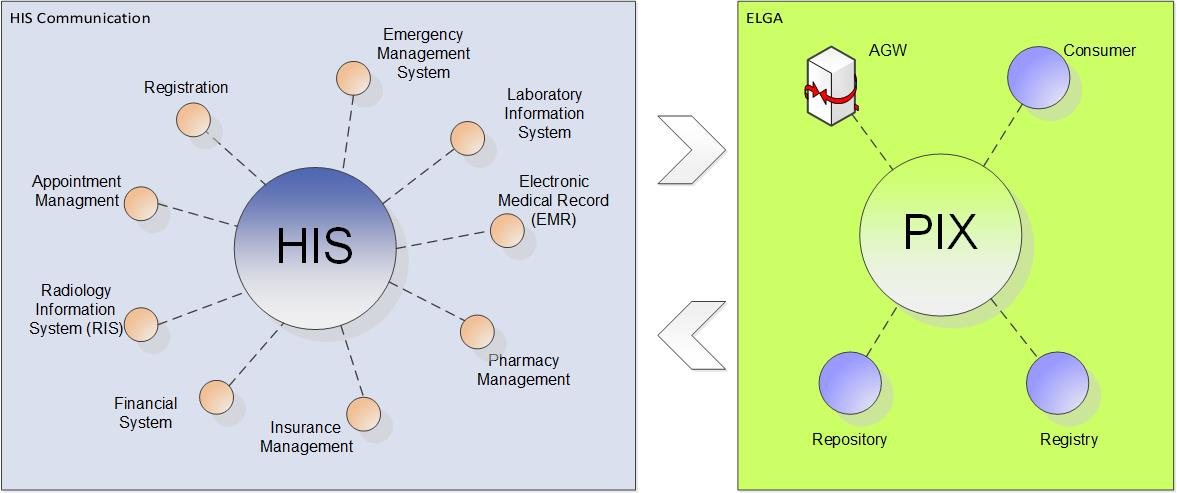
\includegraphics[width=1.0\textwidth]{HIS_Overview}
		  \caption{In the blue box on the left the Hospital Information System
		  Communication can be seen. The HIS  communicates with the ELGA system
		  (on the right) which has its own Patient Identifier Cross Referencing
		  (PIX) and a Access-Gateway (AGW) for connecting and communicating with
		  external partners.}
		\end{figure}
	    Especially in Austria there will be new kind of system for patient-related
	    documents, in which every citizen can restrict access to his data to other
	    parties. The system is called Elektronische Gesundheitsakte (ELGA).
	    This will give the posibility for people in Austria to have a look on their
	    own clinical record in digital way. ELGA and its architecture will be
	    explained in chapter 4.\\
	    To get the systems to speak to each other, a communcation server
	    is used.
	    This Server connects all systems together, map different types of messages
	    in other structered layouts for that they can be understood by other
	    systems and can store messages if destination systems are not available.
	\subsection{Health Level 7}
		The Health Level 7 (HL7) is a standardized protocol in Version 2.5 and in near
		future the Version 3 will be used for communication in eHealth systems.
		All systems, who are communcating in an hospital, are called eHealth
		systems.\\
		HL7 provides a framework to exchange, integrate, share and retrieve 
		electronic health information. It defines also the language, structure and the
		data types which are used for the communicatoin between the eHealth systems.\\
		The standard is human-readable and near to all eHealth systems are able to
		read data from HL7 and export data in HL7.
		
	\newpage
	
	\section{IBM Cognos Business Intelligence}
	IBM Cognos Business Intelligence (BI) is a software suit designed to extract corporate data from data sources,
	whereby a data source is everything from which persistent information could be retrieved. The extracted data
	can be assembled in the Framework Manager environment to build a so called data warehouse. This warehouse forms
	a foundation from which reports could be created and executed in Report Studio. After reports are created Business
	user could run HTML-based Reports in Cognos Webview. Also automation processes and application of user policies,
	restricting access to reports, can be used.
	
	\subsection{Framework Manager}
	The Framework Manager allows the construction of a logic layer, uniting different data sources in terms of 'query
	items', which grant the possiblity of defining customised queries over, for example, multiple tables in one single
	logical item. Also filtering of the retrieved data can be done.
	\subsubsection{Defining Data Sources}
	Before data can be gathered in Framework Manager, database connections have to be made avialable
	for the Cognos application. Since Cognos is running on a windows server, a driver has to be installed for each type
	of database. This can be done in 'ODBC Data Source Administrator'-Tool. When arranging a connection for the first time,
	the appropriate data source type for the connection has to be chosen. This could be ODBC, ANSI or mixed type for 32- and 64 bit. In
	the figure below an existing figure could be seen:\\
	\begin{figure}[!ht]
		  \centering
		      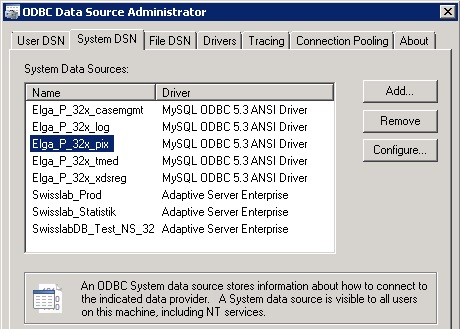
\includegraphics[width=1.0\textwidth]{ExistingDataSource}
		  \caption{}
	\end{figure}
	Furthermore, connection details for the database itself has to be entered for every connection.
	\subsubsection{Frame Manager Surface}
	\hl{Since patient-related Information is used, it must be evaluated how far this information can be revealed.}
	Following figure shows an example of an existing data-warehouse:\\
	\begin{figure}[!ht]
		  \centering
		      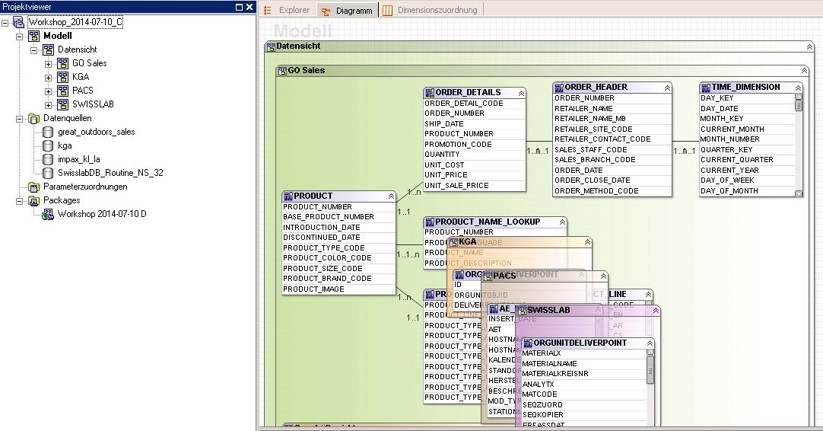
\includegraphics[width=1.0\textwidth]{frameworkM_2}
		  \caption{}
	\end{figure}
	On the left side the project viewer can be seen. It displays in general logical items. This can be data sources,
	views of data sources, which can be modified without altering existing data, and query items. Query items itself
	are highly configurable and allows to define customized and also complex
	queries, which were not possible to execute by selecting data directly.\\
	\\
	Centered, the data view can be seen. It is a graphical surface allowing the
	creation of logic relation beetween tables and query items respectively.
	Filtering of selected data can also be done in this view. With filters
	simply all data can be selected in terms of performance and then limited
	afterwards. This greatly increases perfomance wihtout stressing data sourcs
	Beside the usage of logical relation and filters, also the creation of
	dimensions is possible.
	This can be done in 'Dimensions', which can be seen at the top of the figure. 
	Dimensions allow the comparison of
	Keyfigures dependend on dimensions like time, costs, storage usage and more.\\
	\\
	When the construcion of a data warehous is done or changes on data were
	implemented, a package must be published in order to create reports in Report
	Studio.
	\subsection{Report Studio}
	Report Studio allows the creation of HTML-based reports for end users
	(Business users in Cognos terms), which can be executed on demand or
	time-based.\\
	Follwing figure shows the graphical surface of Report Studio: 
	\begin{figure}[!ht]
		  \centering
		      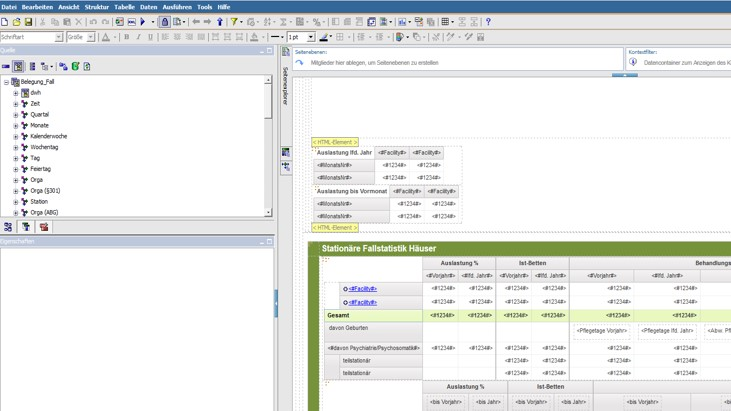
\includegraphics[width=1.0\textwidth]{ReportStudio_2}
		  \caption{}
	\end{figure}
	On the left side query items, dimensions and simple numbers can be seen, which
	were created beforhand in Framework Manager. In the centered view the general
	structure of the report can be assembled by simply drag-and-drop the desired
	elements in the view. Also text, graphical elements and different types of
	diagrams can be added
	\subsection{Data Topology of Cognos}
	As mentioned, Cognos forms a logical data level consisting of
	physical data sources. In Frame Work Manager, query items, dimensions, numbers
	and more can be defined. After the data ware house has been assembled, reports
	can be built in Report Studio and provided to Business Users. This can be seen
	in the following figure:
	\begin{figure}[!ht]
		  \centering
		      \includegraphics[width=1.0\textwidth]{ALLDBtoCognos}
		  \caption{}
	\end{figure}
	
	\newpage
		
	\section{ELGA }
	In the second quarter of year 2016 ELGA in Carinthia (now on referred as 'ELGA Bereich
	K�rnten' (EBK)) will be connected to central core components. This connection will make
	the availability of documents of citizens and 
	also non-citizens possible in entire Austria. Today, the EBK operates
	as a closed unit which receives data solely from carinthian healthcare providers. 
	At this moment no knowledge about quality, correctness and the total amount of data
	exists, which is mainly needed in decision-making processes.\\
	\\
 	This lack of knowledge should be compensated by the use of IBM Cognos Business 
 	Intelligence, a multi-database environment, by creating a data-warehouse in the KABEG-IT
 	department. A data-warehouse forms a model, consisting of several sources of persistent
 	information, and combines them in a central place.\\
 	\\
	The aim of this project is to build up a prototype-model for the ELGA environment from 
	scratch, using the existing databases. On the basis of this model, HTML-based reports 
	for end-users should be created, which should give the actual amount of patients,
	registered documents (locally and also remote ones), queried documents, number 
	of accesses of users and performance of transactions. When the EBK goes live, a distinction
	between regional-ELGA-relevant documents, also called 'Informationsverbund-documents' (IV)
	and EBK-documents will be made. This distinction will also be integrated in reports.\\
	\\
	
	\subsection{XDS - Cross Document Sharing}
	
	The concept of ELGA, in this case IV and EBK, is described by the term Cross Document Sharing
	(XDS), which allows the exchange of documents between healt care providers, also on federal state level.\\
	This requieres following components:\\
	\begin{itemize}
	    	\item PIX - Patient Identifier Cross-Referencing\\
	    	Each ELGA realm uses its own PIX for managing patients. A central patient index is used to
	    	make cross document sharing possbile.
	    	\item Registry\\
	    	IN general the main task of the registry is to link patients with their related information and also documents.
	    	In detail the jobs and funtions of a registry are much more complex. The will be described in PUNKT DATAMODELL VERLINKEN.
	    	\item Policy Repository\\
	    	Access to documents is managed  by a policy repository. The compliance of patients is entered
	    	by care personal, which can be administration personal for example. For EBK-related this process is similiar, but instead
	    	of using the local repository a central authorization system is used. This allows citizens to manage access to their documents
	    	in general and even after their treatment.
	    	\item XDS Repository\\
	    	A repository which consists of multiple logical formed storages. It saves and provides documents
	    	to healt care providers.
	    	\item XDS Consumer\\
	    	A consumer has the role of a client. It retrieves documents from the XDS repository and displays them for users 
	    	\item AGW - Acces Gateway
	    	Main task of the AGW is to connect the EBK to central components and make Cross Community Access (XCA) between
	    	ELGA realms possible.
	    	\item ATNA - Audit Trail and Node Authentication
	    	Every transaction from every node is protocolled in an ATNA repository.
	    	This forms the largest source on which the reports are build on.
	    	
	 \end{itemize}
	
	
	
	\subsection{Data Model}
	The basis structure of the ELGA data model consists of an Electronic Business
	XML - database (ebXML).
	\hl{Will be written as ELGA goes online, since major
	changes to the model will be made.
	Since ELGA handels patient-related data, it must be evaluated how far the model can be described.}
	\subsection{Evaluation and Mesurement of Keyfigures}
	\hl{Will be written as ELGA goes online, since major changes to the model will be made.
	Since ELGA handels patient-related data, it must be evaluated how far the Keyfigures can be described.}
	\subsection{Next Steps}
	Next project steps are the finalization of the prototype-model and the expansion
	of reports. The finalization concerns the investigation of different data-warehouse
	schemes in the aspects of time-efficiency and stress-minimization of the running system.
	The reports will be supplemented with a fraud detection-report, which is supposed to 
	give information about unpermitted- and unregularly access of users. Furthermore,
	several fraud detection techniques will be investigated. As EBK goes online, a major
	update of software and datamodels will be executed, making adaption and changes of the
	existing data-warehouse necessary. On the other hand this can also lead to new possibilities
	for integrating additional information in the data-warehouse.
	
	\newpage
	
	\section{Hospital Information System - AGFA Orbis}
	The Hospital Information System forms the center in inter-clinical
	communication. All patient data will be stored in this system and every booking
	and timebased terms for patients will also be made here.\\
	In the KABEG there are five hospitals and two different Hospital Information
	Systems in total. In the future, a major change will be made, so that only one
	HIS is in use in KABEG organisations. This will be solely AGFA Orbis.
	\subsection{Orbis in the KABEG}
	At the moment, only four of five KABEG hospitals are useing AGFA Orbis as HIS.
	The main functionality of Orbis is to collect all patient data and distribute
	them to all subsystems. Beside its main task, Orbis has much more
	functionalities.\\
	Orbis consits of many modules which are connected together to one system. One
	of this module is an appointment calender system. Here the users can plan
	patient appointments and additional events but the calender can also be used
	for internal scheduls and notes.
	Another module is the planing and documentation of surgeries. In this module
	the users have a view about all operating rooms and can see when patients
	are coming in, when did the surgery starts and ends and much more.\\
	\begin{figure}[!ht]
		  \centering
		      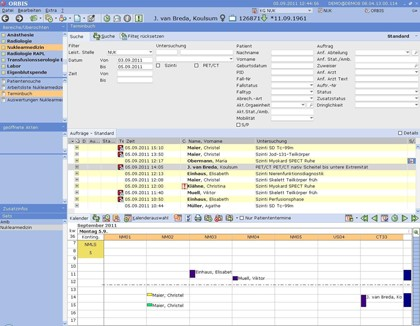
\includegraphics[width=0.6\textwidth]{orbis1}
		  \caption{Orbis Appointment calender system. User can plan 
		  patients appointments and their own terms.}
	\end{figure}
	A third module is a planing module for orders of radiological
	examinations. There the users can order examinations and this will trigger an
	order on X-ray units and other devices. Also available in Orbis is an 
	overview about the clinical history of all patients. There are
	stored values of laboratory investigations, links to medical reports, which are
	stored in the Electronical Medical Record, and much more.\\
	In many other Hospital Information Systems all the features above are not
	available and so for every additional requierement another subsystem will be
	used.
	This is great advantage of Orbis. On the other hand, one disadvantag of orbis
	is that nearly all of these modules were productes of smaller companies which
	were regrated from AGFA. Many modules were migrated to Orbis and and its
	overall-performance suffers from it and is not as well as the users wish.
	This can be seen in the Orbis database which is described in the next chapter.\\
	\begin{figure}[!ht]
		  \centering
		      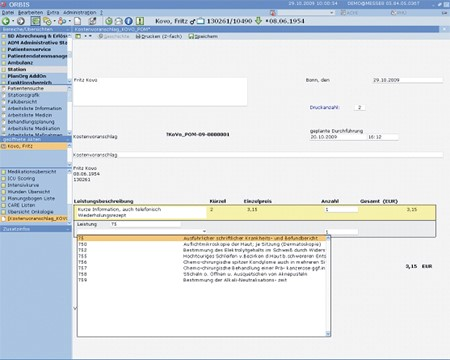
\includegraphics[width=0.6\textwidth]{orbis2}
		  \caption{Orbis Module for diagnosis and medical reports. There users can
		  select the diagnosis from a defined catalogue and write a free text to the
		  medical report which is stored as a PDF file in the Electronical Medical
		  Record.}
	\end{figure}
	\subsection{Orbis Database}
	The Orbis Database has grown over years. At the beginning it was a small
	Database for a small application to store patientdata. Because of many user
	wishes the company AGFA has to build in new features. \\
	\begin{figure}[!ht]
		  \centering
		      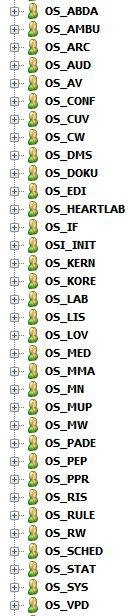
\includegraphics[width=0.12\textwidth]{orbis_db_schema}
		  \caption{Overview about the Orbis Database Schemes.}
	\end{figure}
	On one hand they developed some new features and modules for the application
	and on the second they buy some applications or the company, which develope the
	application directly and merge them to Orbis. So the database became more and
	more and also new schemes and tables were added. Which leads to the main
	problem: a good performance for users.
	\subsection{Actual Problems}
	The actual problem is that many database models were merged together. Many of
	them are not state of the art. So there are really big Database tables with
	many columns and without primary keys. They also don't have foreign keys to
	other other necessary tables. So sometimes it is not easy to get the right
	value to make a join over different tables.\\
	Another problem is get a general overview about Orbis-Database, also because of
	the problems described above. This makes it nessecary to get and define
	simple values, which are displayed in the application as well. Deep
	knowledge of the Orbis-database is necessary. It is not
	a simple matter to get performant and correct asserting from Orbis.
	\subsection{Reports for Orbis}
	It was a goal of the project to build reports for boards of directors of the
	Orbis database in IBM Cognos. 
	\subsubsection{Overview about the reports}
	A Cognos Cube was build with AGFA and an automatically server job was developed
	to get actual data from the Orbis Database to this Cognos Cube.\\
	The next step was to use the IBM Cognos Report Studio to develope reports for
	the Web-Browser in HTML and for the iPhone application.
	\begin{figure}[!ht]
		  \centering
		      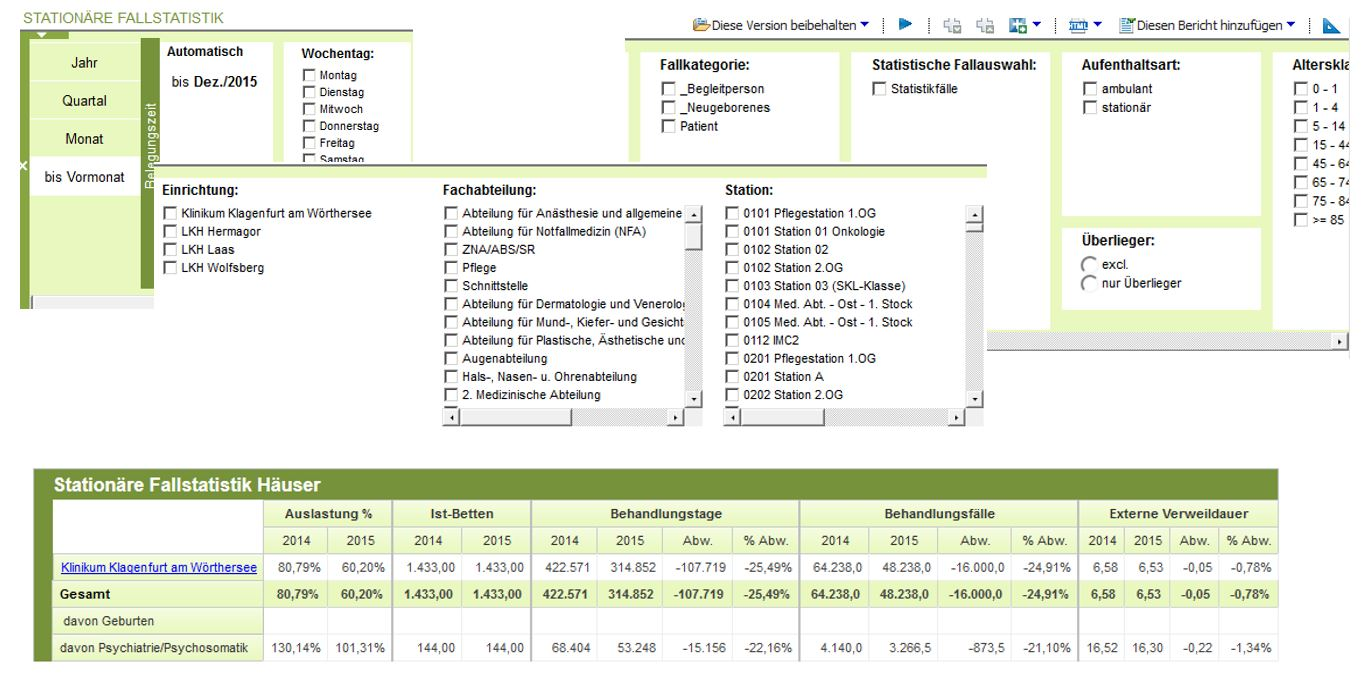
\includegraphics[width=1.0\textwidth]{reports_overview}
		  \caption{An overview about one of the reports. It is
		  possible to select the hospital, department and station and more. It is
		  also important to get a selection about in- or outgoing-patient and the
		  timeline and much other properties. The board of directors will get an
		  overview about the statistics they want and can select the properties on
		  their own.}
	\end{figure}
	\subsubsection{Result of the report}
	The results of the reports, which the boards of directors will get from it,
	where displayed in tables, charts and diagrams. So it will be simple for them
	to present statistical key figueres from the Hospital Information System and the
	billing and other statistics.
	\begin{figure}[!ht]
		  \centering
		      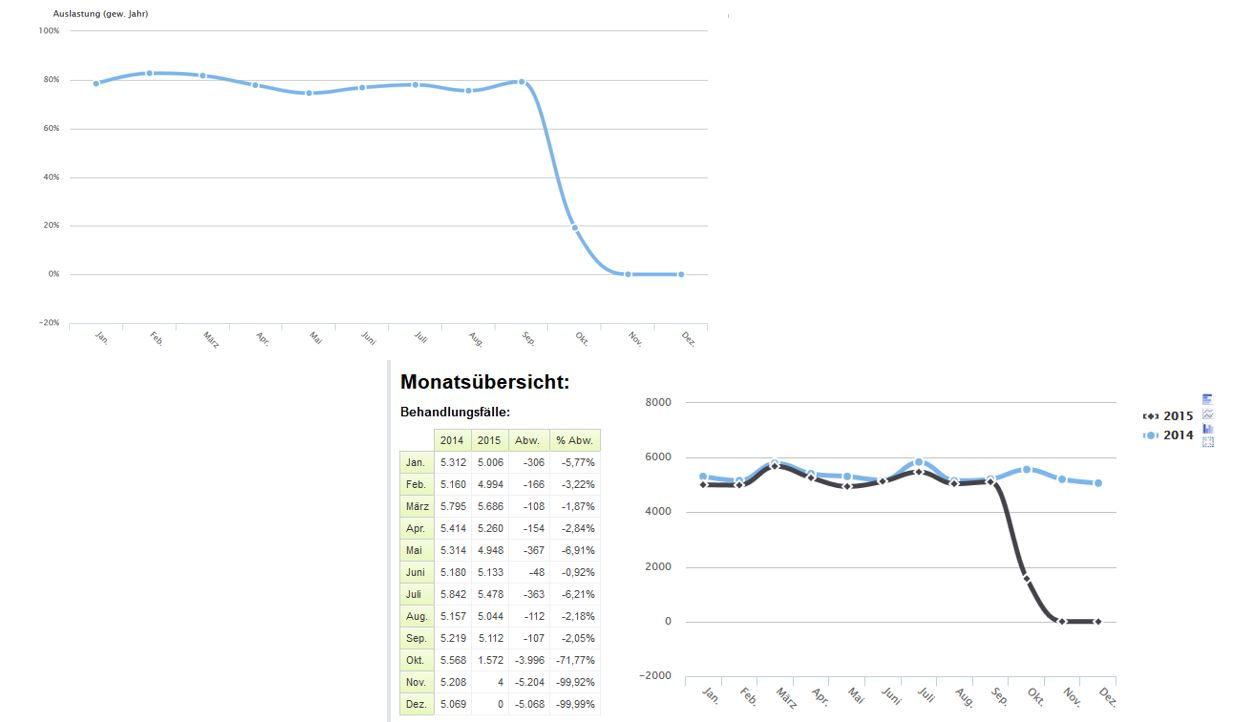
\includegraphics[width=1.0\textwidth]{reports_results}
		  \caption{An Example for a report for the in-patient statistic of the
		  Klinikum Klagenfurt. The load factor of the Klinikum is shown. It is
		  obvious the curve decreases to Zero on October. This is because the data
		  which were displayed for this tests are available ot October in the Cognos
		  Cube.}
	\end{figure}

\end{document}
